\documentclass[review]{elsarticle}

\usepackage{lineno,hyperref}
\modulolinenumbers[5]

\journal{International Journal of Forecasting}

%%%%%%%%%%%%%%%%%%%%%%%
%% Elsevier bibliography styles
%%%%%%%%%%%%%%%%%%%%%%%
%% To change the style, put a % in front of the second line of the current style and
%% remove the % from the second line of the style you would like to use.
%%%%%%%%%%%%%%%%%%%%%%%

%% Numbered
%\bibliographystyle{model1-num-names}

%% Numbered without titles
%\bibliographystyle{model1a-num-names}

%% Harvard
%\bibliographystyle{model2-names.bst}\biboptions{authoryear}

%% Vancouver numbered
%\usepackage{numcompress}\bibliographystyle{model3-num-names}

%% Vancouver name/year
%\usepackage{numcompress}\bibliographystyle{model4-names}\biboptions{authoryear}

%% APA style
%\bibliographystyle{model5-names}\biboptions{authoryear}

%% AMA style
%\usepackage{numcompress}\bibliographystyle{model6-num-names}

%% `Elsevier LaTeX' style
\bibliographystyle{elsarticle-num}
%%%%%%%%%%%%%%%%%%%%%%%

\begin{document}

\begin{frontmatter}

\title{Ensemble forecasts of COVID-19 cases and deaths in the United States}

%% or include affiliations in footnotes:
\author[umass,mysecondaryaddress]{Evan L. Ray\corref{mycorrespondingauthor}}
\cortext[mycorrespondingauthor]{Corresponding author}
\ead{elray@umass.edu}

\author[cmu]{Logan C. Brooks}

\author[umass]{Yijin Wang}

\author[umass]{Aaron Gerding}

\author[umass]{Estee Cramer}

\author[umass]{Martha Zorn}

\author[usc]{Jacob Bien}

\author[kit,hits]{Johannes Bracher}

\author[cmu]{Aaron Rumack}

\author[cdc]{Matthew Biggerstaff}

\author[cdc]{Michael A. Johansson}

\author[cmu]{Ryan J. Tibshirani}

\author[umass]{Nicholas G. Reich}

\address[umass]{School of Public Health and Health Sciences, University of Massachusetts Amherst}
\address[cmu]{Machine Learning Department, Carnegie Mellon University}
\address[usc]{Department of Data Sciences and Operations, University of Southern California}
\address[kit]{Chair of Econometrics and Statistics, Karlsruhe Institute of Technology}
\address[hits]{Computational Statistics Group, Heidelberg Institute for Theoretical Studies}
\address[cdc]{COVID-19 Response, U.S. Centers for Disease Control and Prevention}

\begin{abstract}
Abstract goes here.
\end{abstract}

\begin{keyword}
COVID-19\sep forecast\sep ensemble\sep keyword 4
\MSC[2010] 00-01\sep  99-00
\end{keyword}

\end{frontmatter}

\linenumbers

\section{Introduction}

\begin{itemize}
  \item General overview
  \begin{itemize}
    \item Forecasts of short-term trajectory can help inform public health response.
    \item Ensemble forecasts are generally performant
    \item We consider how to effectively construct ensemble forecasts of the short-term trajectory of COVID-19 to support public health end users.
  \end{itemize}
  \item Review literature on ensemble forecasting in general and for infectious disease in particular
  \item Review literature on ensemble methodology
  \begin{itemize}
    \item quantile averaging and density averaging
    \item exponentially weighted averaging (weights are sigmoid of a measure of forecast skill)
  \end{itemize}
  \item Summary of our motivations and contributions
  \begin{itemize}
    \item Goal is to produce ensemble forecasts of short-term trajectory of COVID-19 that have good average performance and stable performance across time and locations.
    \item Real-time forecasting introduces challenges that we need to be able to handle; most importantly,
    \begin{itemize}
      \item Outlying component forecasts due to software errors or difficulties handling data reporting anomalies
      \item Missing component forecasts from teams that join at different times or submit forecasts for a subset of locations
      \item mention other things?
    \end{itemize}
    \item We explore and compare variations on ensemble methods designed to address these challenges by using combination mechanisms that are robust to outliers and may allow for giving more weight to better component forecasters.
  \end{itemize}
\end{itemize}

\section{Context and Analysis Set Up: forecasting COVID-19 burden in the United States}

\begin{itemize}
  \item Describe hub and parameters of our analysis
  \begin{itemize}
    \item Dates active, geographic scales, forecast targets, representation in terms of quantiles
    \item In this analysis, we focus on state level forecasts of incident deaths between July 27, 2020 and May 31, 2021 and forecasts of incident cases between ... and May 31, 2021.
  \end{itemize}
  \item Exhibit features of component forecasts that motivate our methods
  \begin{itemize}
    \item Occasional outlying forecasts motivate robust methods
    \item Some component forecasters are consistently better than others; motivates trained methods
  \end{itemize}
  \item Figure with data and component/ensemble forecasts?
\end{itemize}

\section{Methods}

\begin{itemize}
  \item Approaches to evaluation
  \begin{itemize}
    \item WIS/pinball loss
    \item relative WIS to handle missingness
  \end{itemize}
  \item Two-by-two table with methods we primarily consider:
  \begin{itemize}
    \item equal-weighted mean
    \item equal-weighted median
    \item weighted mean
    \item weighted median, based on relative WIS
  \end{itemize}
  \item Details about trained methods that we will consider in the primary analysis
  \begin{itemize}
    \item Training set window size: 4, 8, 12, or "full history" weeks
    \item Number of component forecasters included: all eligible, top 10, or top 5
    \item Handle missing forecasts by setting their weight to 0 and "renormalizing"
  \end{itemize}
  \item Other details for which careful exploration is deferred to the supplement
  \begin{itemize}
    \item Introduce extra parameters for each forecast horizon? (or, turn this around and use per-horizon weights in the main analysis and simplified version in supplement?)
    \item Introduce extra parameters for each quantile level (or for 3 groups of quantile levels)?
  \end{itemize}
\end{itemize}

\section{Results}

\begin{figure}
  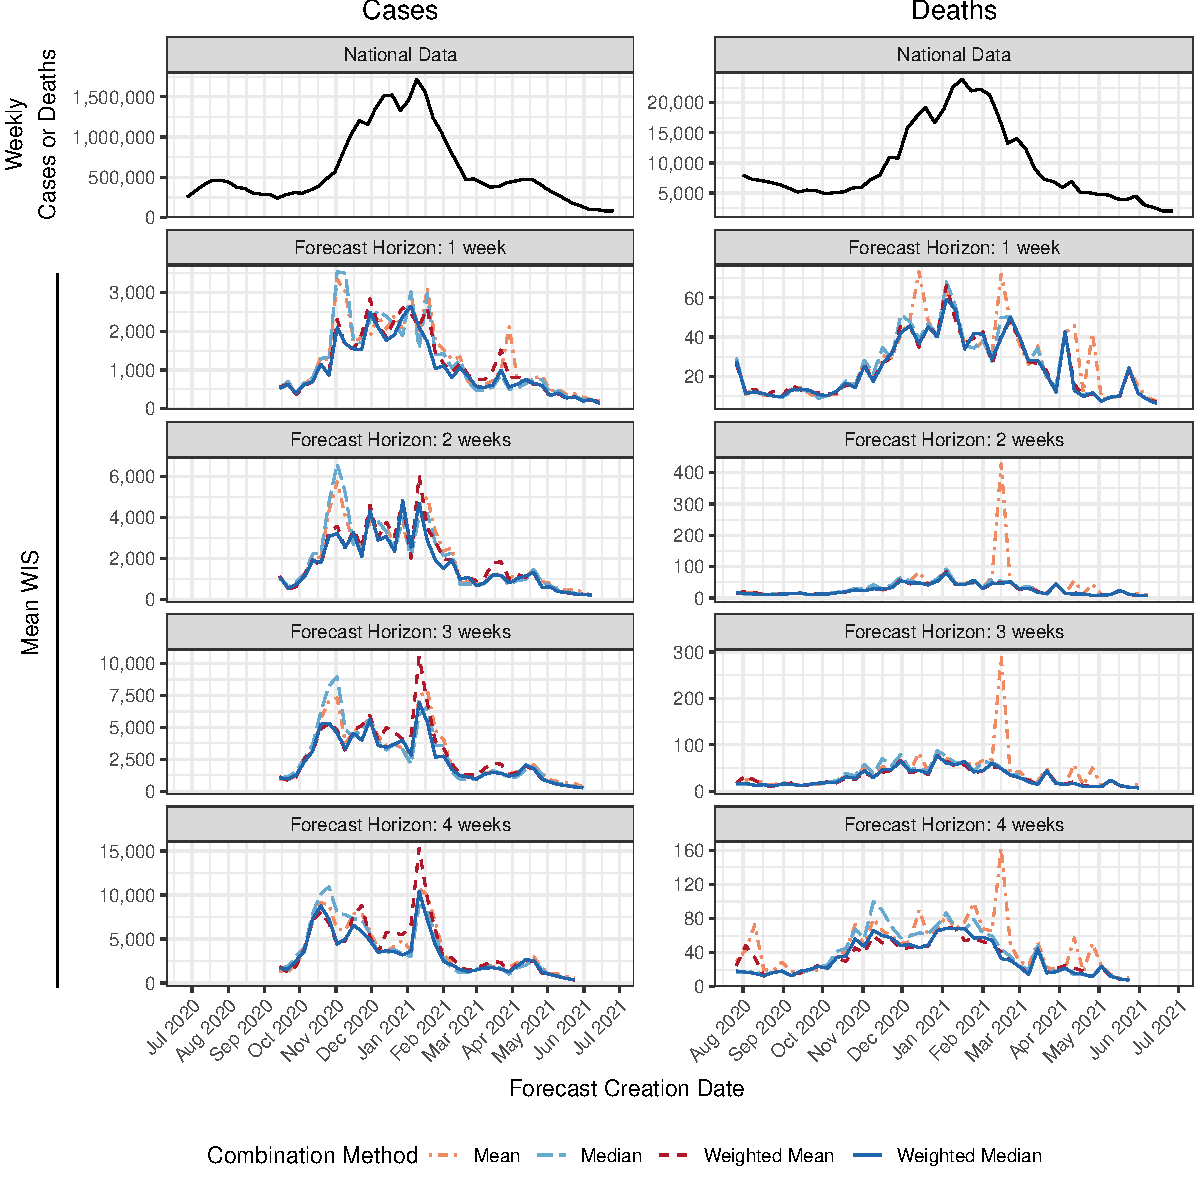
\includegraphics[width=\textwidth]{figures/scores_by_week.pdf}
  \caption{Weekly reported cases and deaths at the national level and mean weighted interval scores (WIS) for state-level forecasts over time for four ensembles:
  1) an equally weighted mean ensemble, 2) an equally weighted median ensemble, 3) a weighted mean ensemble, and 4) a weighted median ensemble.
  Both of the weighted ensembles combine the ten component forecasters with best individual performance as measured by the relative WIS, and are trained on a sliding 12-week window.
  The component forecasters included in the trained ensembles each week are updated each week based on performance during the training window.
  Means are calculated separately for each combination forecast horizon and forecast creation date, averaging across all states and territories.
  Lower scores indicate better forecast performance.}
  \label{fig:WIS_over_time}
\end{figure}

\begin{figure}
  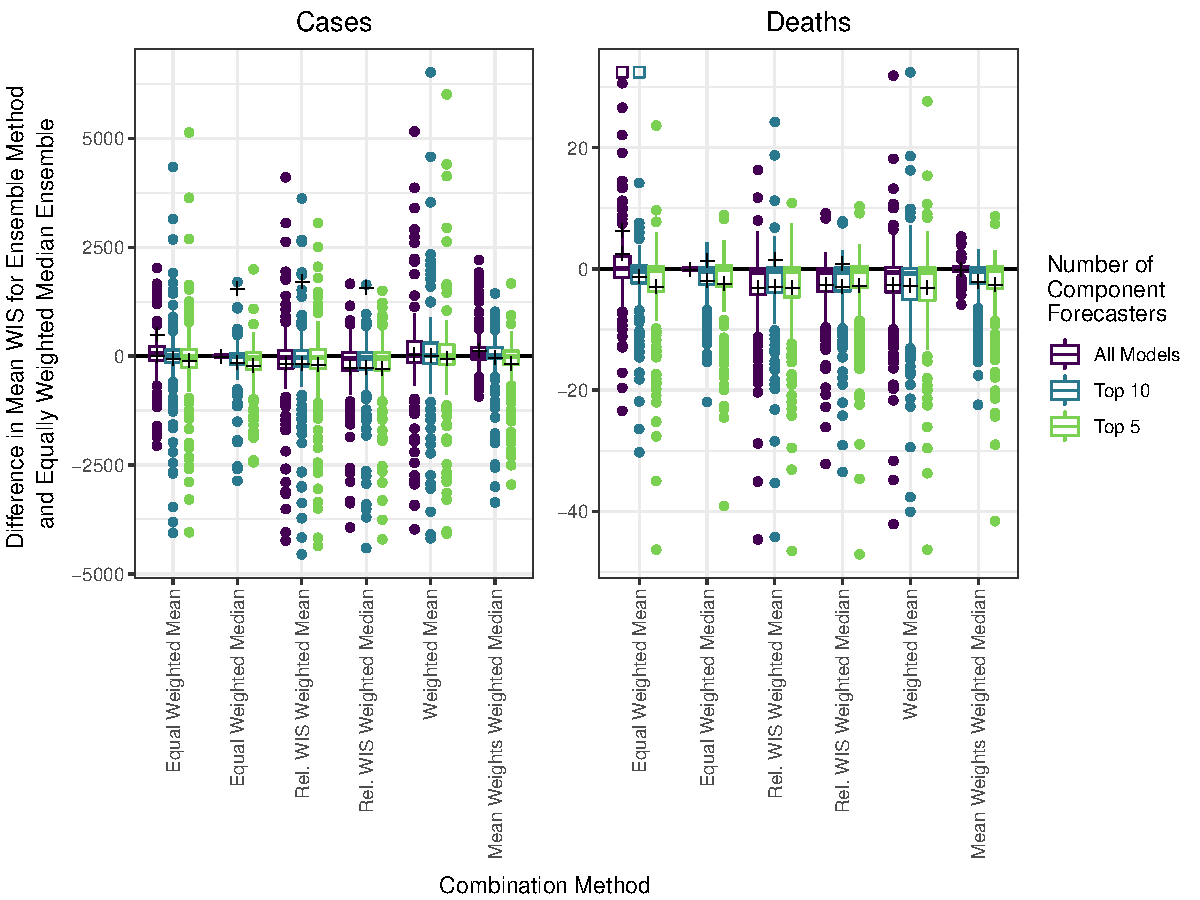
\includegraphics[width=\textwidth]{figures/wis_boxplots_main.pdf}
  \caption{Boxplots summarizing forecast skill for forecasts of weekly cases (top row) and deaths (bottom row).
  The vertical axis is the difference in mean skill for the given method and the equally-weighted median;
  the boxplots summarize the distribution of these differences for each combination of forecast date and horizon, averaging across all locations.
  A cross is displayed at the difference in mean scores for the specified combination method and the equally weighted median.
  A negative value indicates that the given method outperformed the equally weighted median.
  Columns indicate the size of the training set, and colors indicate the number of component forecasters included in the ensemble.
  For readability of the plot, four large outliers for the equally weighted mean ensemble forecasts of incident deaths are truncated, indicated with a hollow square point.}
  \label{fig:overall_WIS_boxplots}
\end{figure}

\begin{figure}
  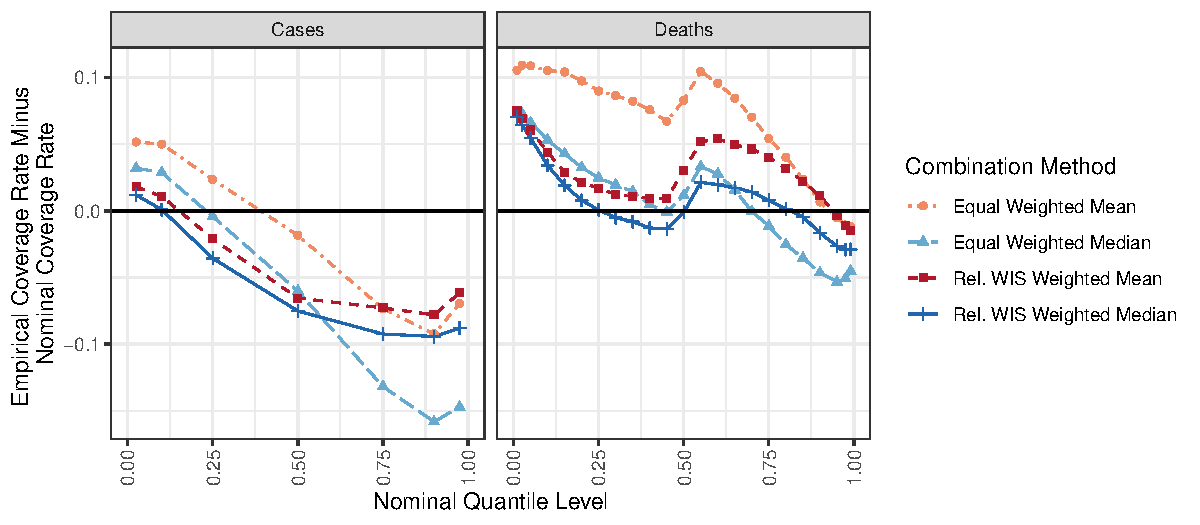
\includegraphics[width=\textwidth]{figures/quantile_coverage_main.pdf}
  \caption{Quantile coverage rates for ensemble forecasts of weekly reported cases and deaths. The horizontal axis gives the nominal quantile level of the prediction; there are seven quantile levels for forecasts of cases and 23 quantile levels for forecasts of deaths.
  The vertical axis gives the empirical coverage rate of the forecasts at each quantile level, calculated as the proportion of eventually observed values that were less than or equal to the predictive quantile.
  A well calibrated model will have empirical coverage rates approximately equal to the nominal quantile level.}
  \label{fig:quantile_coverage_main}
\end{figure}

\begin{itemize}
  \item Figures \ref{fig:overall_WIS_boxplots} and \ref{fig:quantile_coverage_main} display summaries of overall performance across all locations, forecast dates, and forecast horizons.  The main take aways are:
  \begin{itemize}
    \item Robust methods are helpful:
    \begin{itemize}
      \item Comparison of equally-weighted approaches: For both incident cases and incident deaths, the equally weighted median had better mean and worst-case weighted interval scores than the equally weighted mean.  However, the equally-weighted median ensemble did have lower coverage rates in the upper tail than the equally-weighted mean ensemble.
      \item Comparison of weighted approaches: The relative WIS weighted median was generally at least as good as the weighted mean; differences in mean WIS between these methods were more pronounced for cases than for deaths.  Even for cases, there were more outliers in values of WIS for the weighted mean approach, where skill was substantially worse than the equally-weighted median approach.  For trained approaches, the weighted median had almost strictly better probabilistic calibration than the trained mean.  For the weighted mean approach, subsetting to top-performing models led to improved calibration, but there were not corresponding gains from subsetting to fewer forecasters when using the weighted median ensemble. This may be because the weighted median approach has fewer parameters to estimate, and so is less likely to overfit the training data.
    \end{itemize}
    \item Trained methods can have improved mean performance, with caveats
    \begin{itemize}
      \item In our evaluations for incident cases and deaths, averaging across all forecasts, the weighted median was better than equally-weighted median and weighted mean was better than equally-weighted mean.  These improvements were especially pronounced during times of stable trends that many component forecasters did not capture.
      \item But there are some specific times when the weighted approaches were not as good as an equally-weighted median.  Specifically, trained methods have more of a tendency to "miss" at turning points by predicting a continuation of recent trends.
    \end{itemize}
  \end{itemize}
  \item Although the magnitude of scores was larger at larger forecast horizons, these general trends in the relative performance of different ensemble specifications were stable across different forecast horizons (Supplemental Figures 1 and 2).
  \item For both trained ensembles, using separate model weights at each forecast horizon led to some small improvents in forecast skill at short term forecast horizons of 1 and 2 weeks ahead, but generally worse forecast skill at longer forecast horizons of 3 and 4 weeks ahead (Supplemental Figures 3 and 4).  These differences in forecast skill were more pronounced for the weighted mean ensemble than for the weighted median ensemble.
  \item Performance for the trained median was not very sensitive to other details of the ensemble specification.
  \begin{itemize}
    \item improvements in mean skill of the weighted median were consistent across target variables (incident cases and deaths) and choices for training set window size and number of component forecasters included (Figure~\ref{fig:overall_WIS_boxplots}).
    \item Allowing for separate parameters per quantile level had limited impact for the weighted mean approach, but was unhelpful for the weighted median (Supplemental Figures ...).  Note that reductions in coverage concentrated in a few times. Need to make some plots to try to understand what was happening.
    \item We also considered other possible formulations of a weighted median, including fitting an unweighted median to a subset of top-performing models and calculating the weighted median using the weights that were obtained from the weighted mean.  As measured by WIS, the best versions of these other variations on weighted medians had similar performance to the best versions of the relative WIS weighted median considered in the primary analysis.  However, the method using weights transferred from a weighted mean ensemble was more sensitive to settings like the number of component forecasters included (Supplemental Figure ...).
  \end{itemize}
\end{itemize}

\section{Discussion}

\begin{itemize}
  \item Robust methods are helpful
  \item Trained methods can have improved mean performance, with caveats
  \item Important note: our analysis uses forecasts and ground truth data as they were available in real time, but it is not a prospective analysis.  We examined a large number of methods and selected a few to discuss here.  Our results should be taken as a statement of how these methods would have done over the past year, and we do not necessarily claim that these findings generalize to the future.
  \item Summary: robust methods are appealing for public health end users.
\end{itemize}

\section{Supplemental Materials (to be moved to a separate file once we're confident about what goes where)}

\subsection{Scores broken down by forecast horizon}

\begin{figure}
  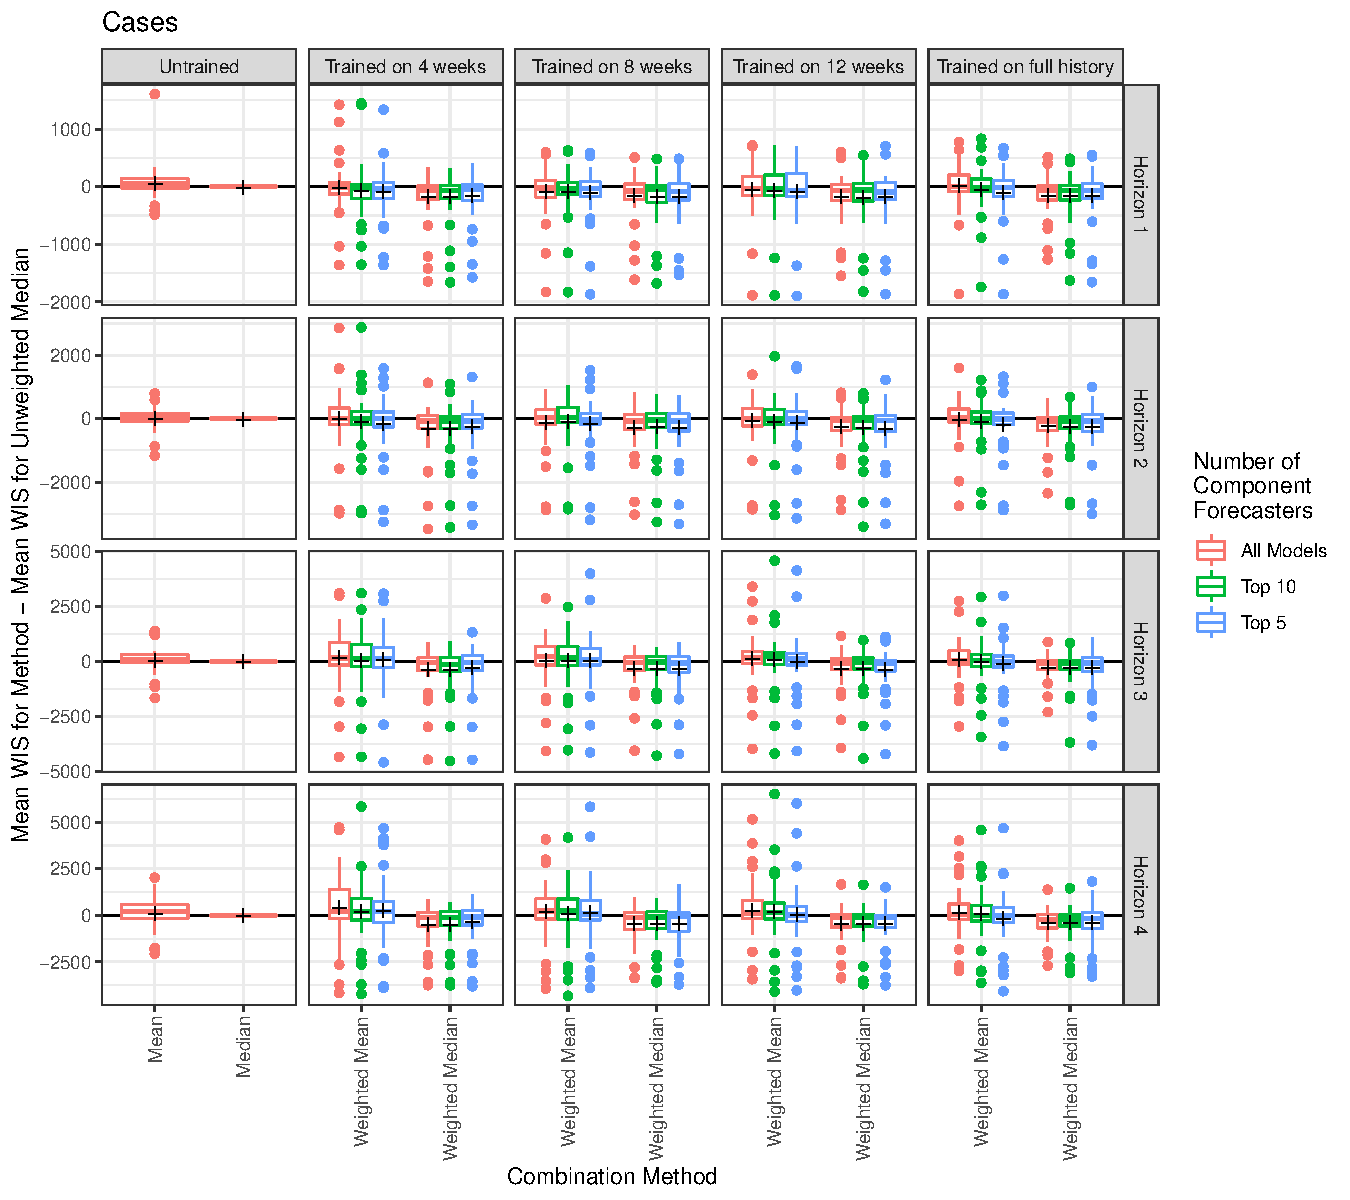
\includegraphics[width=\textwidth]{figures/wis_boxplots_main_by_horizon_Cases.pdf}
  \caption{Boxplots summarizing forecast skill for forecasts of weekly cases, broken down by forecast horizon (in rows).
  The vertical axis is the difference in mean skill for the given method and the equally-weighted median;
  the boxplots summarize the distribution of these differences for each combination of forecast date and horizon, averaging across all locations.
  A cross is displayed at the difference in mean scores for the specified combination method and the equally weighted median.
  A negative value indicates that the given method outperformed the equally weighted median.
  Columns indicate the size of the training set, and colors indicate the number of component forecasters included in the ensemble.
  For readability of the plot, four large outliers for the equally weighted mean ensemble forecasts of incident deaths are truncated, indicated with a hollow square point.}
\end{figure}


\begin{figure}
  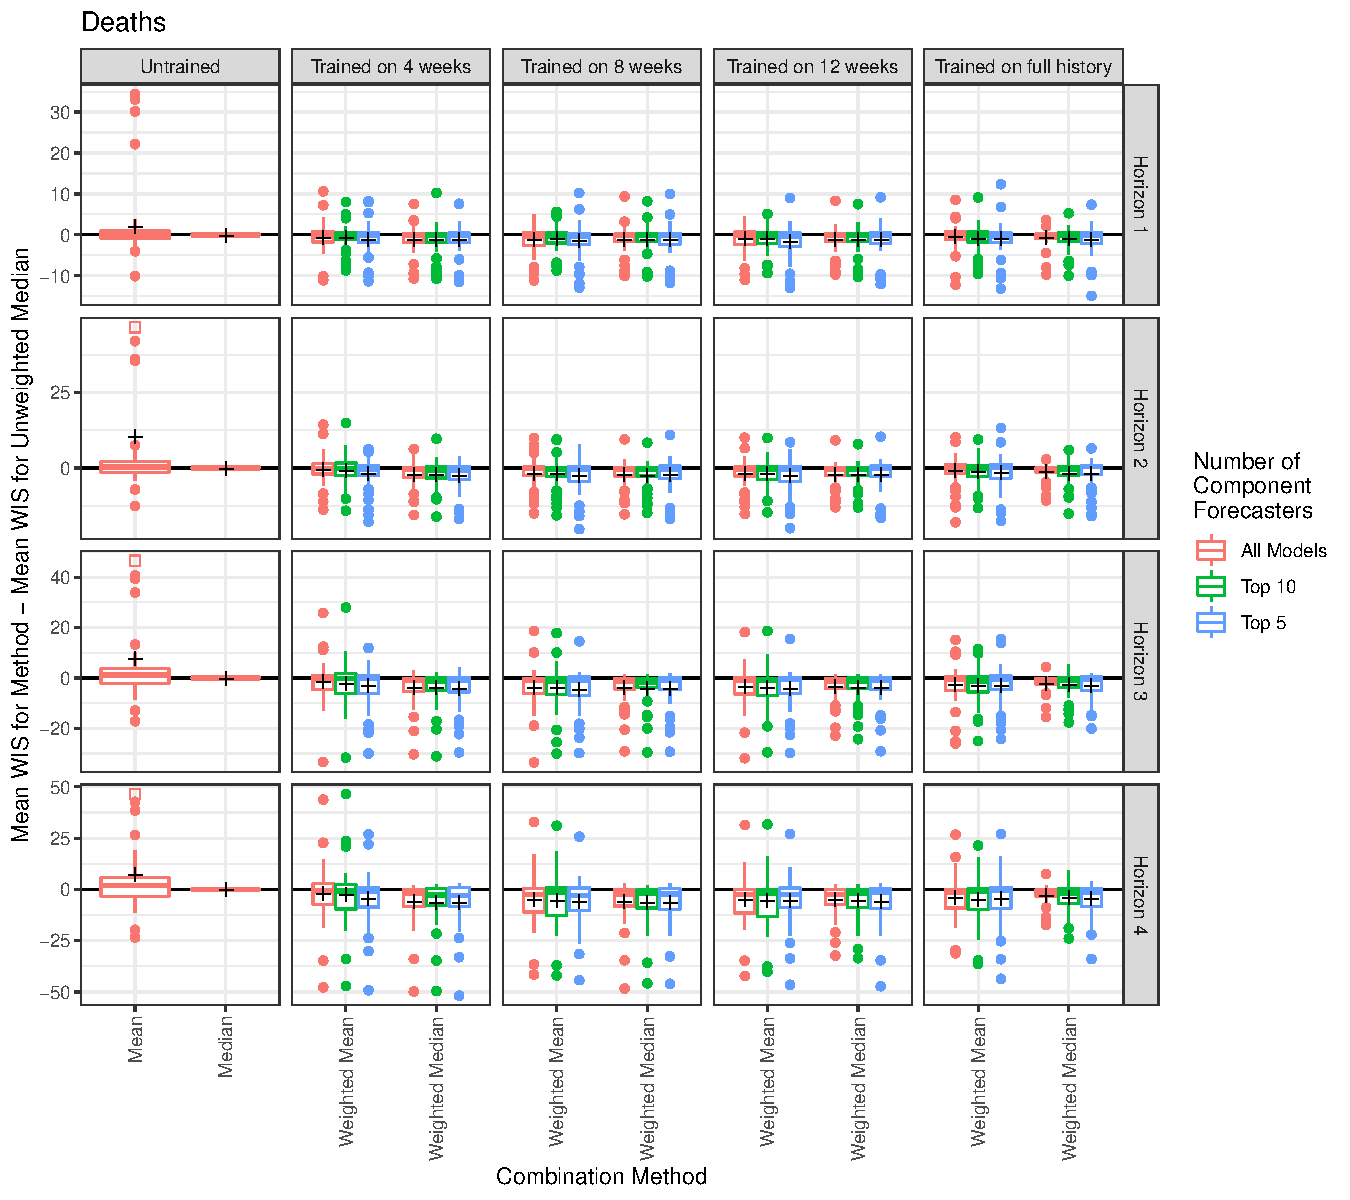
\includegraphics[width=\textwidth]{figures/wis_boxplots_main_by_horizon_Deaths.pdf}
  \caption{Boxplots summarizing forecast skill for forecasts of weekly deaths, broken down by forecast horizon (in rows).
  The vertical axis is the difference in mean skill for the given method and the equally-weighted median;
  the boxplots summarize the distribution of these differences for each combination of forecast date and horizon, averaging across all locations.
  A cross is displayed at the difference in mean scores for the specified combination method and the equally weighted median.
  A negative value indicates that the given method outperformed the equally weighted median.
  Columns indicate the size of the training set, and colors indicate the number of component forecasters included in the ensemble.
  For readability of the plot, four large outliers for the equally weighted mean ensemble forecasts of incident deaths are truncated, indicated with a hollow square point.}
\end{figure}

\subsection{Separate weights at different forecast horizons}

\begin{figure}
  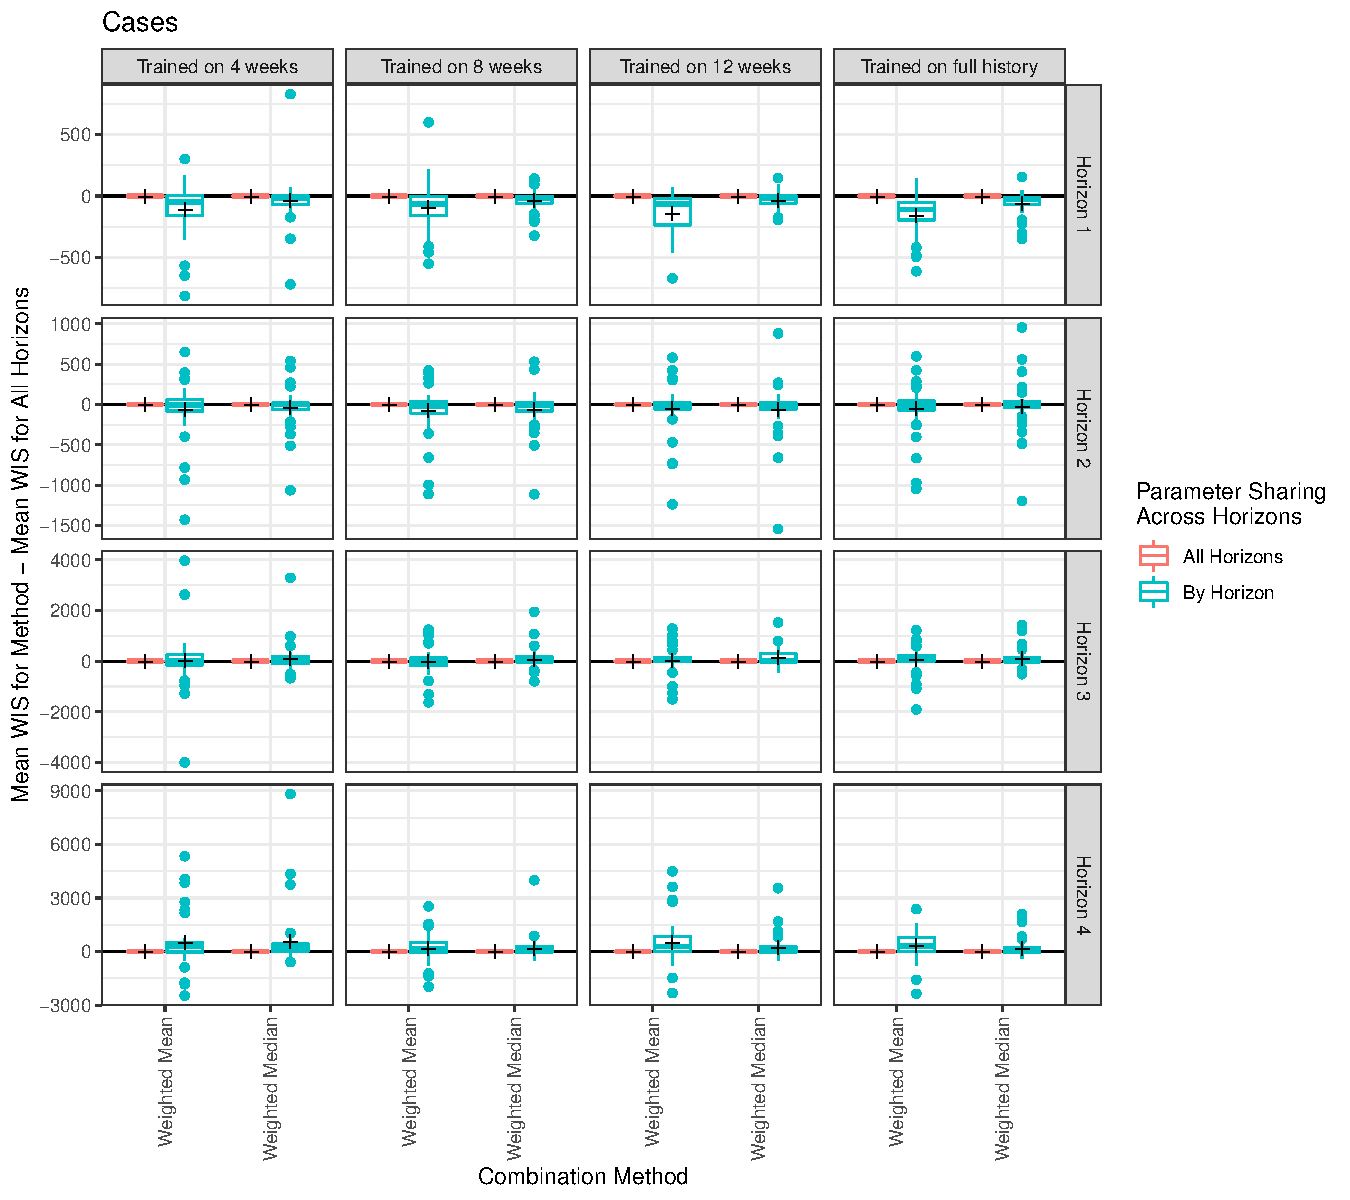
\includegraphics[width=\textwidth]{figures/wis_boxplots_horizon_grouping_Cases.pdf}
  \caption{Boxplots summarizing forecast skill for forecasts of weekly cases, varying whether model weights are shared across all forecast horizons or are estimated separately for each forecast horizon.
  The vertical axis is the difference in mean skill for the given ensemble specification when component weights are shared across all horizons and the same specification with separate component weights for each forecast horizon.
  The boxplots summarize the distribution of these differences for each combination of forecast date and horizon, averaging across all locations.
  A cross is displayed at the difference in overall mean scores.
  A negative value indicates that the method with separate component weights for each forecast horizon outperformed the corresponding specification with weights shared across forecast horizons.
  For this analysis, only results for trained ensembles combining the ten best individual component forecasters are presented.
  Columns indicate the size of the training set.}
\end{figure}


\begin{figure}
  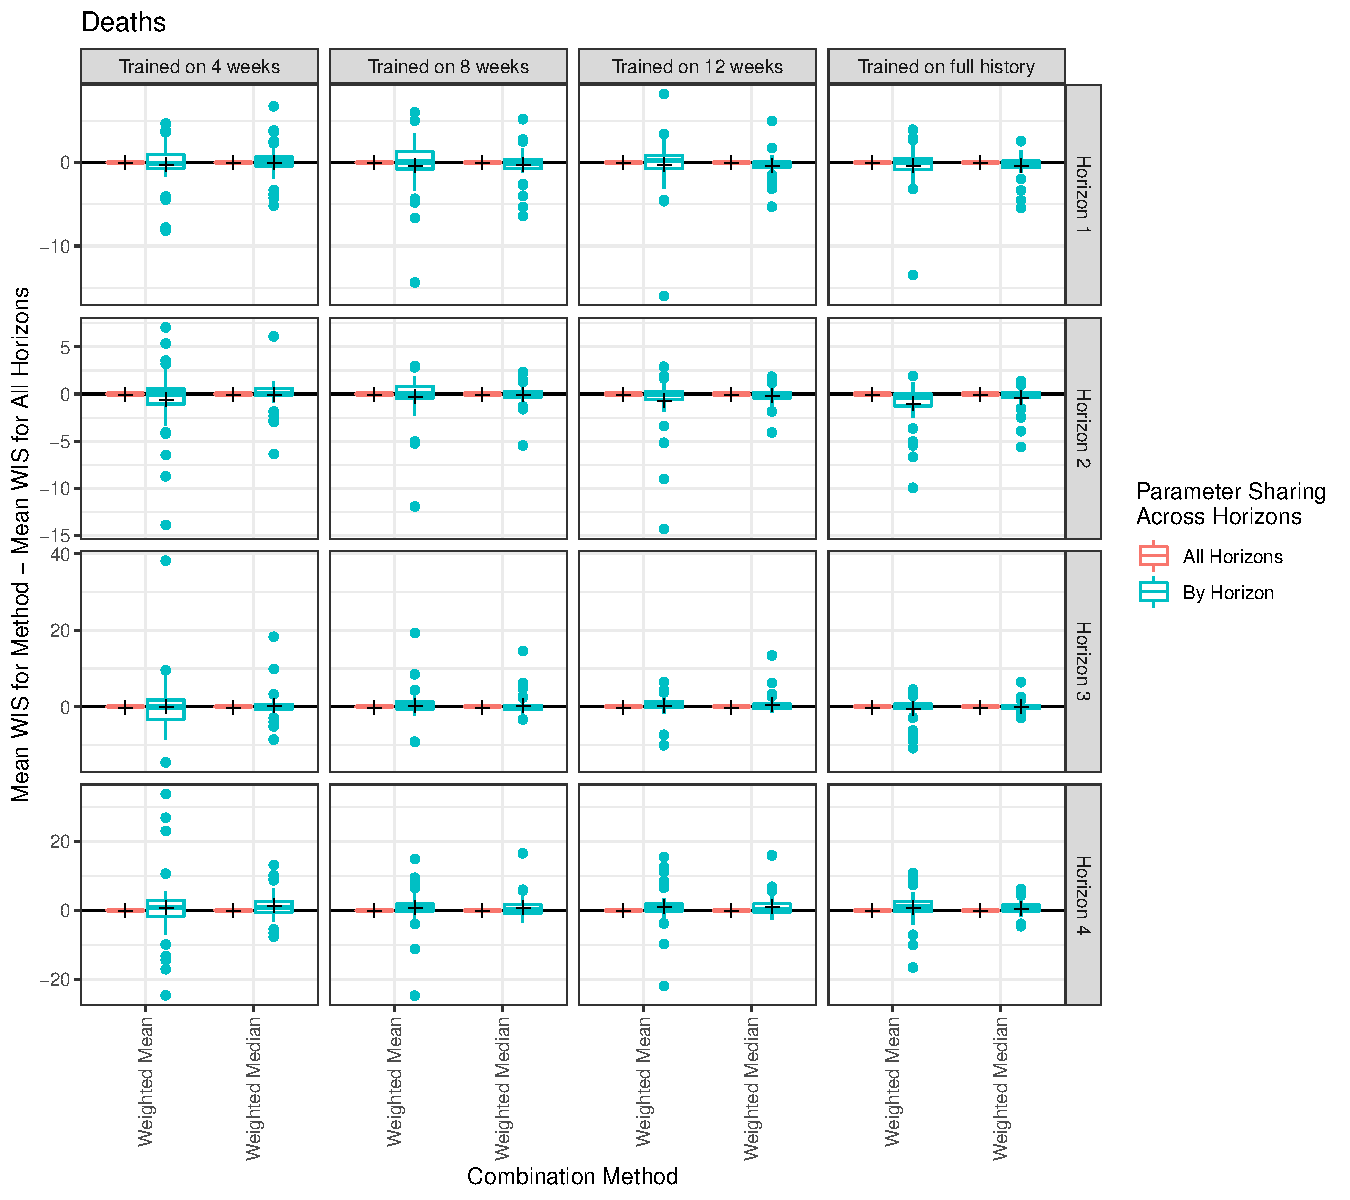
\includegraphics[width=\textwidth]{figures/wis_boxplots_horizon_grouping_Deaths.pdf}
  \caption{Boxplots summarizing forecast skill for forecasts of weekly deaths, varying whether model weights are shared across all forecast horizons or are estimated separately for each forecast horizon.
  The vertical axis is the difference in mean skill for the given ensemble specification when component weights are shared across all horizons and the same specification with separate component weights for each forecast horizon.
  The boxplots summarize the distribution of these differences for each combination of forecast date and horizon, averaging across all locations.
  A cross is displayed at the difference in overall mean scores.
  A negative value indicates that the method with separate component weights for each forecast horizon outperformed the corresponding specification with weights shared across forecast horizons.
  For this analysis, only results for trained ensembles combining the ten best individual component forecasters are presented.
  Columns indicate the size of the training set.}
\end{figure}


\subsection{Separate weights at different quantile levels}


\begin{figure}
  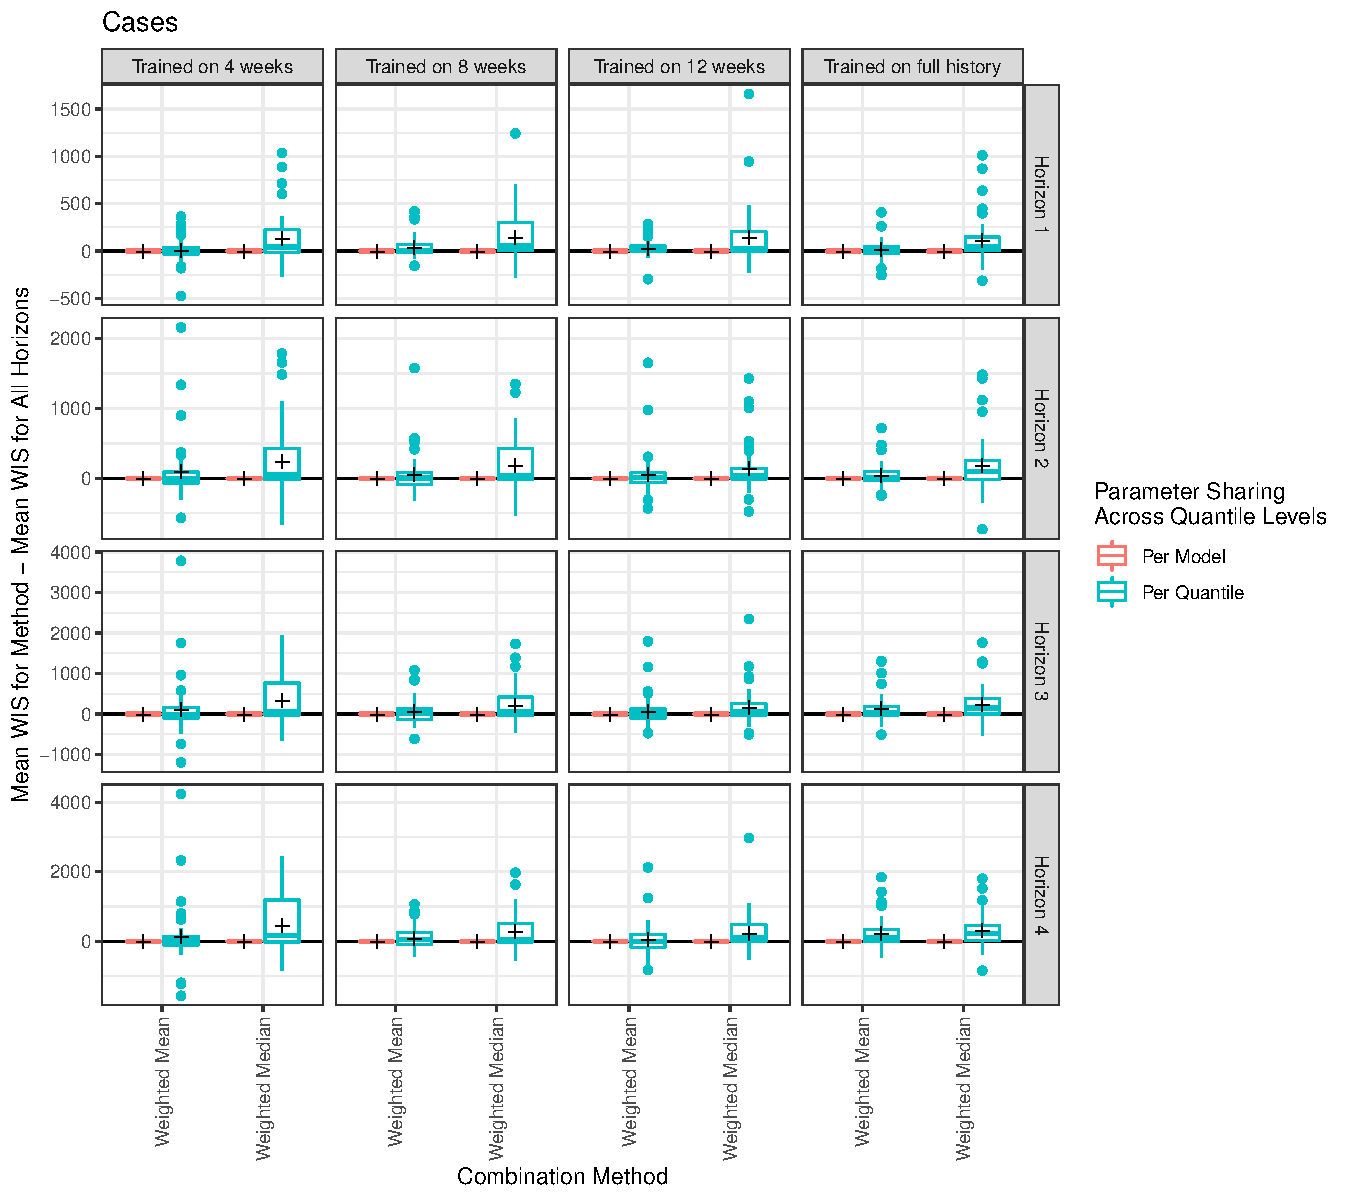
\includegraphics[width=\textwidth]{figures/wis_boxplots_quantile_grouping_Cases.pdf}
  \caption{Boxplots summarizing forecast skill for forecasts of weekly cases, varying whether model weights are shared across all quantile levels or are estimated separately for each quantile level.
  The vertical axis is the difference in mean skill for the given ensemble specification when component weights are shared across all quantile levels and the same specification with separate component weights for each quantile level.
  The boxplots summarize the distribution of these differences for each combination of forecast date and horizon, averaging across all locations.
  A cross is displayed at the difference in overall mean scores.
  A negative value indicates that the method with separate component weights for each quantile level outperformed the corresponding specification with weights shared across quantile levels.
  For this analysis, only results for trained ensembles combining the ten best individual component forecasters are presented.
  Columns indicate the size of the training set.}
\end{figure}


\begin{figure}
  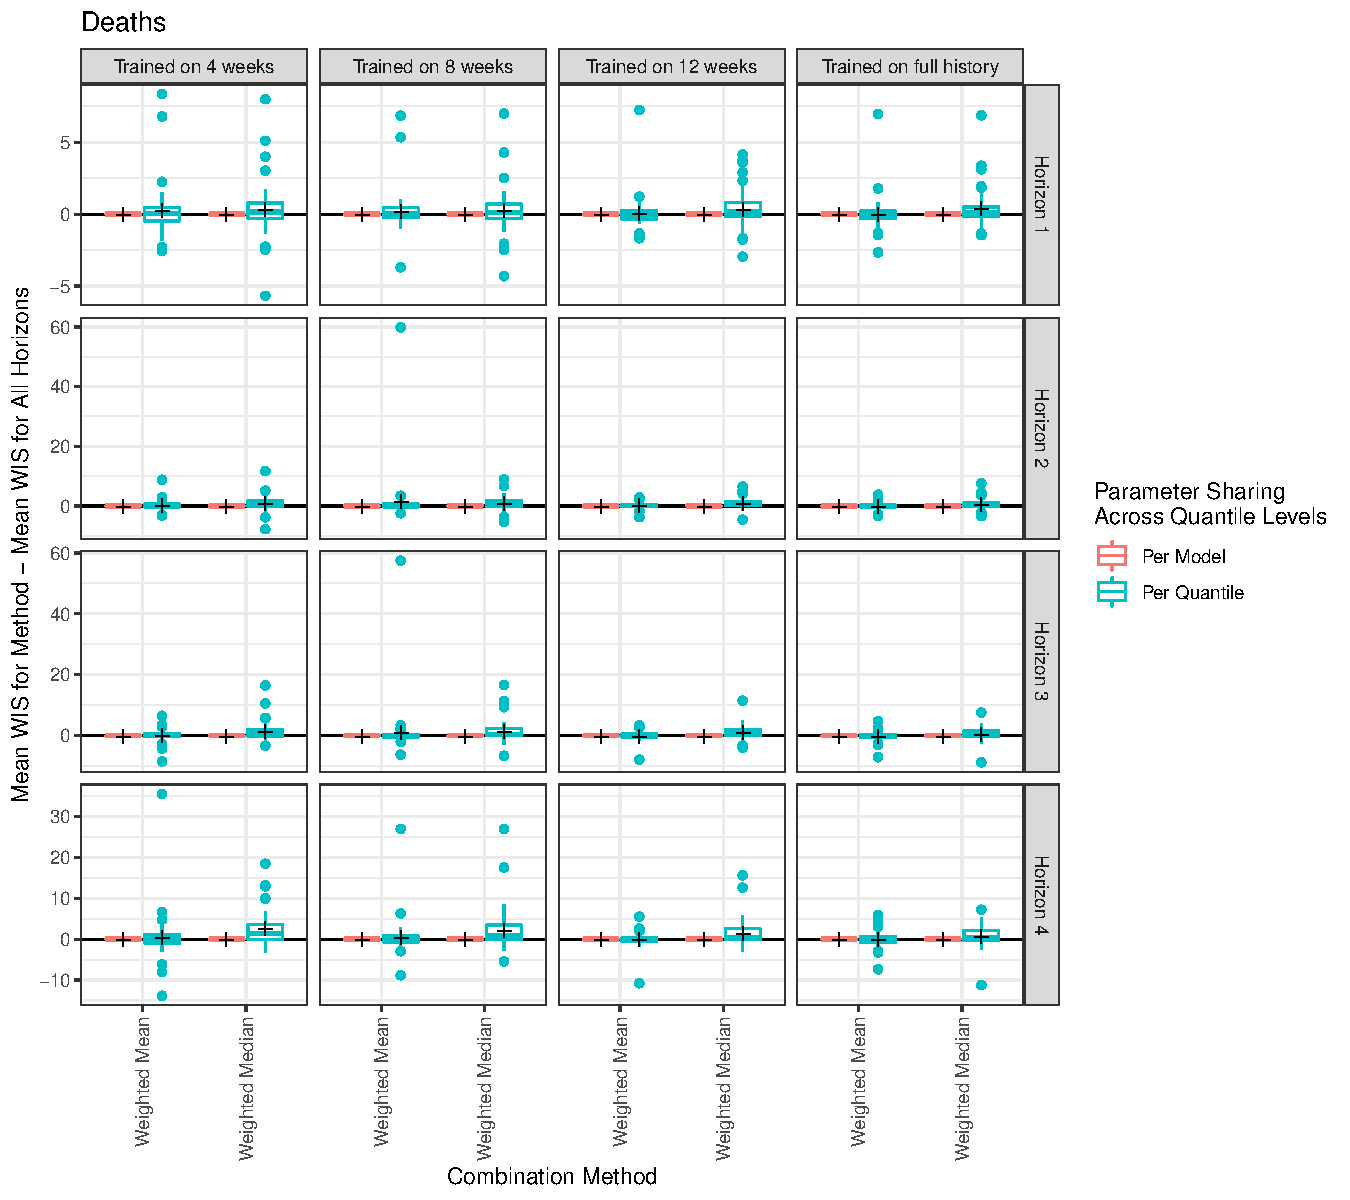
\includegraphics[width=\textwidth]{figures/wis_boxplots_quantile_grouping_Deaths.pdf}
  \caption{Boxplots summarizing forecast skill for forecasts of weekly deaths, varying whether model weights are shared across all quantile levels or are estimated separately for each quantile level.
  The vertical axis is the difference in mean skill for the given ensemble specification when component weights are shared across all quantile levels and the same specification with separate component weights for each quantile level.
  The boxplots summarize the distribution of these differences for each combination of forecast date and horizon, averaging across all locations.
  A cross is displayed at the difference in overall mean scores.
  A negative value indicates that the method with separate component weights for each quantile level outperformed the corresponding specification with weights shared across quantile levels.
  For this analysis, only results for trained ensembles combining the ten best individual component forecasters are presented.
  Columns indicate the size of the training set.}
\end{figure}




\begin{figure}
  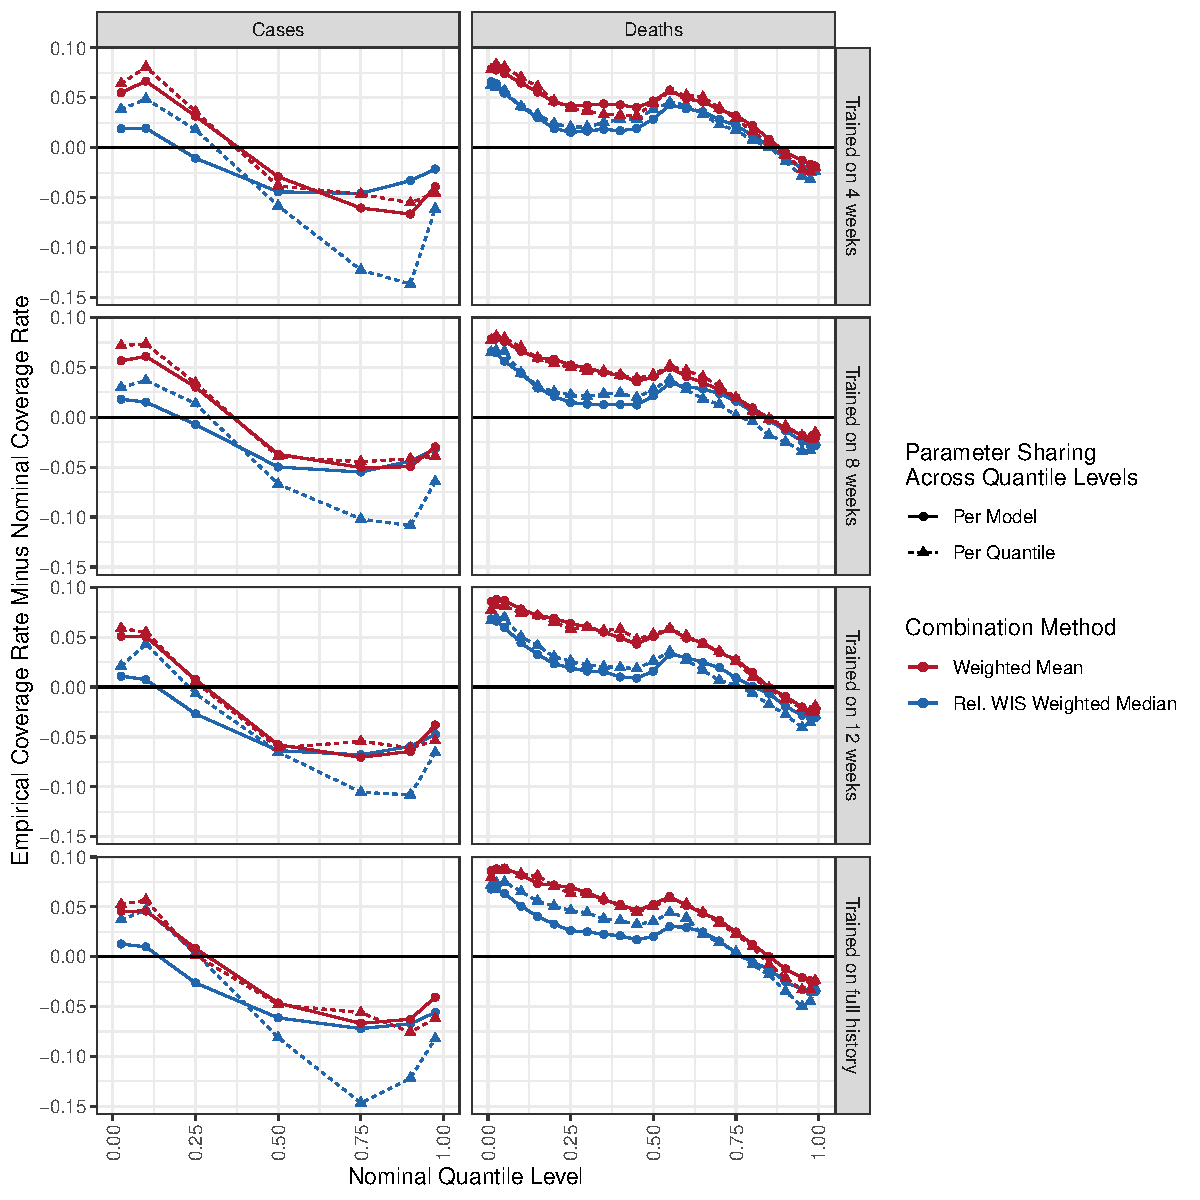
\includegraphics[width=\textwidth]{figures/quantile_coverage_quantile_group.pdf}
  \caption{Quantile coverage rates.}
\end{figure}


\begin{figure}
  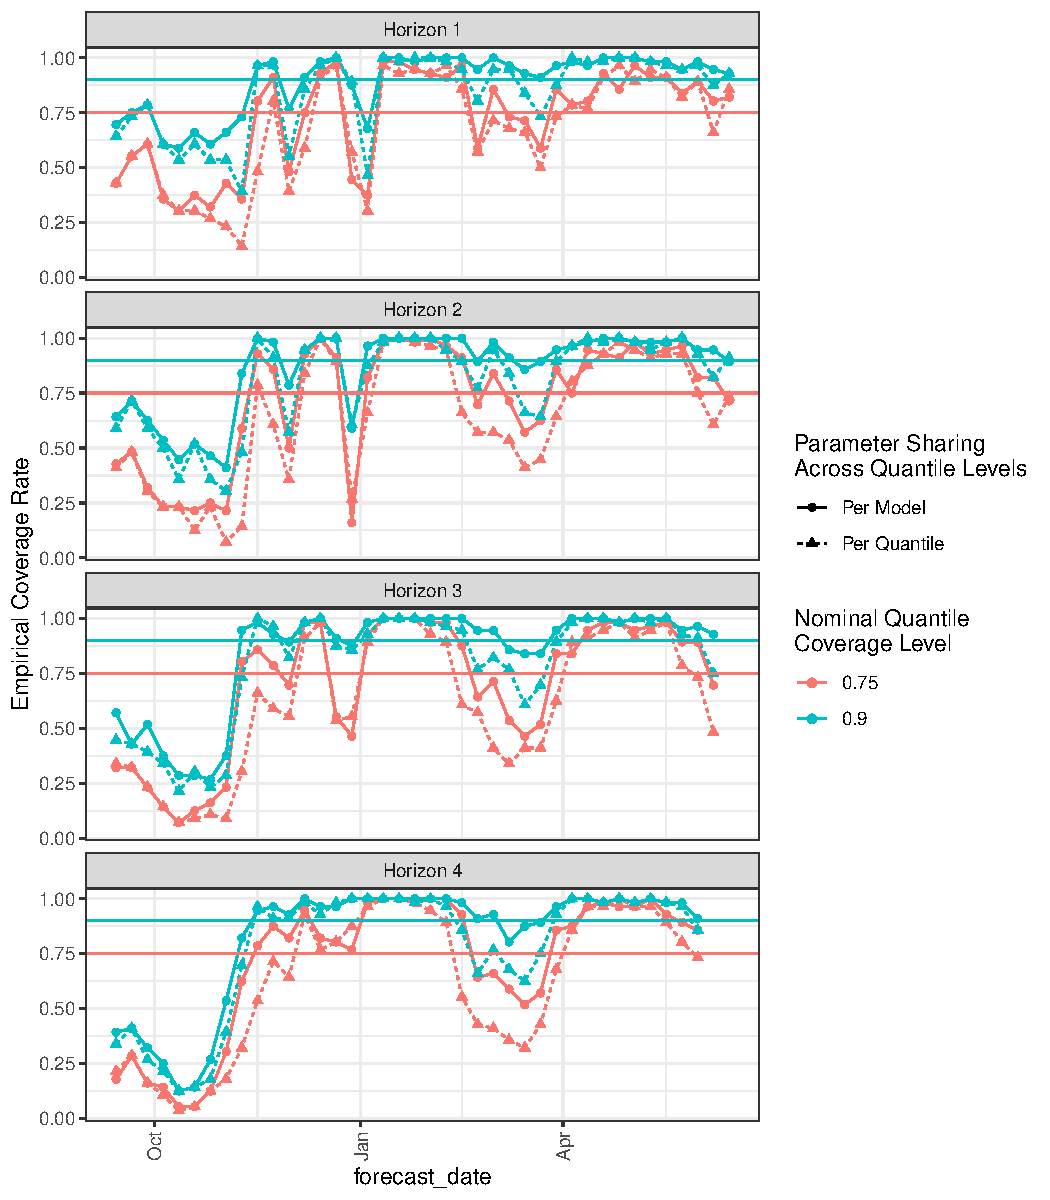
\includegraphics[width=\textwidth]{figures/quantile_coverage_quantile_group_by_date_Cases.pdf}
  \caption{Quantile coverage rates over time.}
\end{figure}



\subsection{Impact of reporting anomalies}

Nothing here yet.  Preliminary examinations indicate "not much".

\subsection{Other approaches to weighted medians}


\begin{figure}
  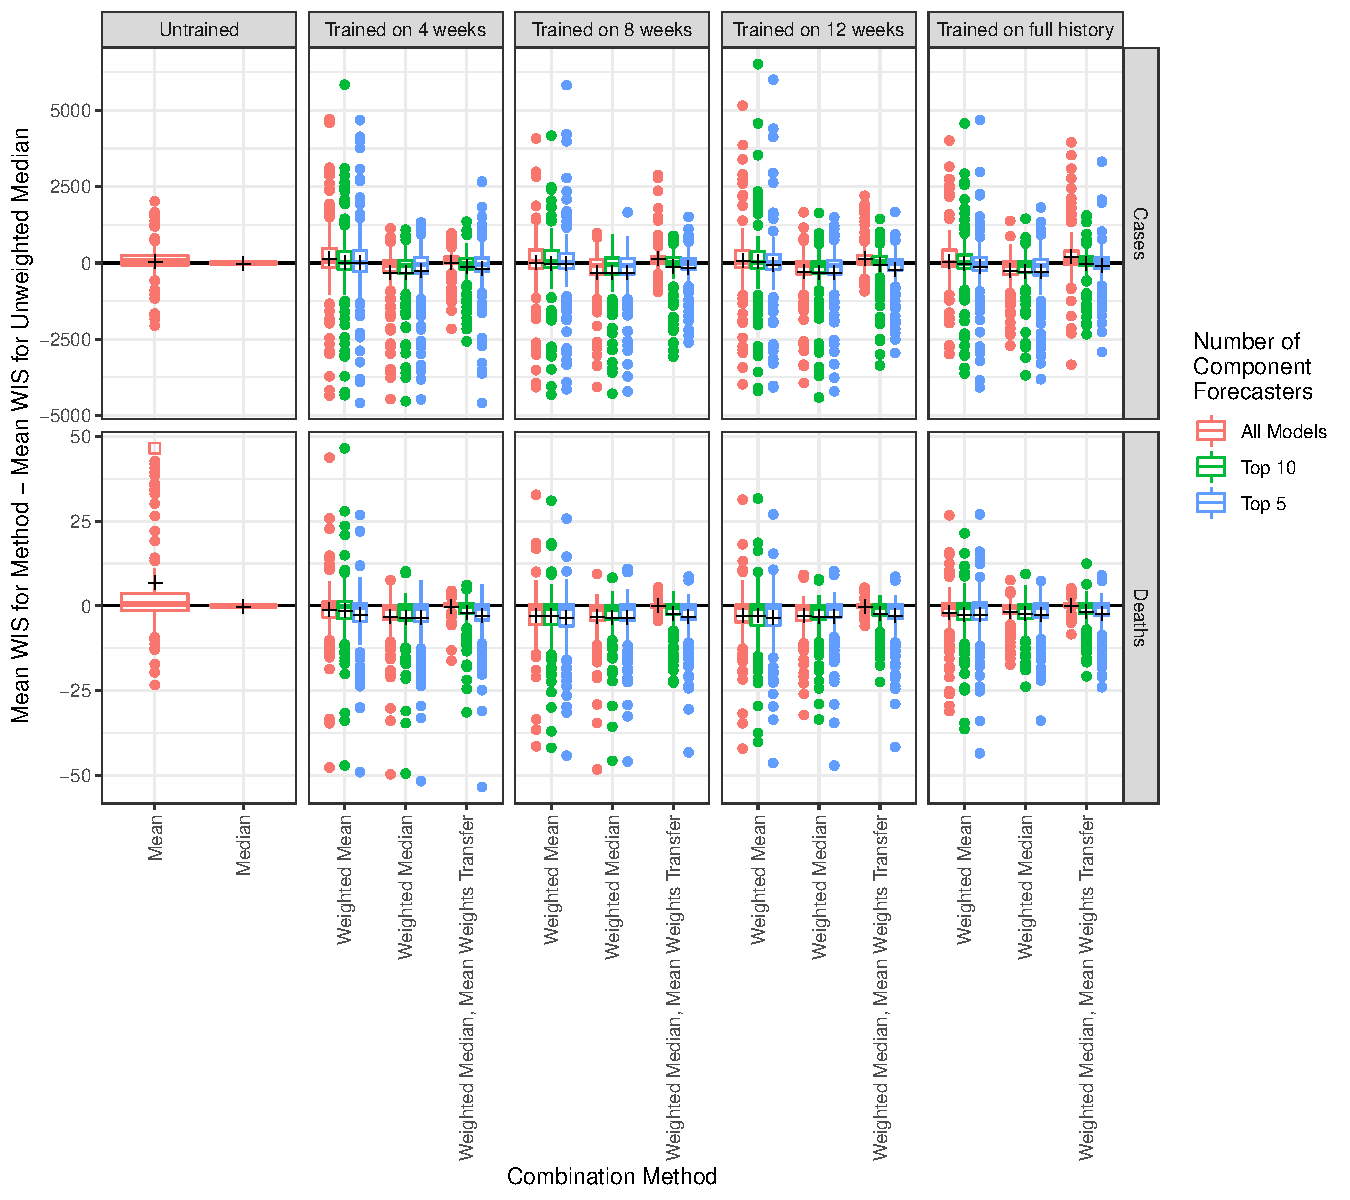
\includegraphics[width=\textwidth]{figures/wis_boxplots_all_combine_methods.pdf}
  \caption{WIS boxplots including additional variations on weighted medians.  Need to add equally-weighted median of individual top-performing models back into the mix here.}
\end{figure}



\begin{itemize}
  \item Approaches we have tried -- generally similar to the relative WIS weighted approach presented in the main text, occasionally a little worse.
  \begin{itemize}
    \item Equally-weighted median of best component forecasters
    \item Transfer weights from weighted mean to weighted median -- similar to the relative WIS weighted approach
  \end{itemize}
  \item Estimate weighted median weights directly -- challenging computationally, Ryan has offered to write this up.
\end{itemize}

\section*{References}

\bibliography{bibfile}

\end{document}